% The "%" character denotes a comment
% This file was written by Nathan Moore, Winona State University
% as a template for how lab reports might be written in LaTeX.
% style choices originally come from the American Journal of Physics's
% sample submission file, http://ajp.dickinson.edu/Contributors/manFormat.html
%
%
\documentclass[prb,preprint]{revtex4-1}
\usepackage{amsmath}  % needed for \tfrac, \bmatrix, etc.
\usepackage{amsfonts} % needed for bold Greek, Fraktur, and blackboard bold
\usepackage{graphicx} % needed for figures

%these are some macros (shortcuts)
\newcommand{\bea}{\begin{eqnarray}}
\newcommand{\eea}{\end{eqnarray}}
\newcommand{\be}{\begin{equation}}
\newcommand{\ee}{\end{equation}}

\begin{document}

\title{Electronics Lab 04: Operational Amplifiers - Frequency vs. Gain}
\author{Adam Stammer}
%\email{adam.stammer@go.winona.edu}

\date{\today}

%if you include an abstract, it goes here
\begin{abstract}
Not Requested
\end{abstract}

\maketitle


%These are my general reccomendations for an undergraduate lab report in Physics. 
%
%\textbf{Purpose}
%The lab report should start with a purpose statement.  Briefly 
%provide the necessary background and explain what problem your are trying to 
%solve/investigate.
%
%\textbf{Conclusions} Don't be coy, cut to the point right away and state what you found. This should be breif.
%
%\textbf{Theory} We never just measure stuff in Physics.  There's always a 
%theoretical idea behind the measurement we're making.  Explain  the ideas 
%behind your work, starting at the level of a successful Physics 221/222 
%student.
%
%\textbf{Data} Sketch out, in words and pictures, the apparatus you used to take data.  Report the data, graphically, if possible, and state the uncertainties  in your measurement.  Don't provide pages of computer printout here. Data tables shouldn't be your first choice when it comes to communicating your measurements.\cite{Tufte}
%
%\textbf{Analysis} With data presented, describe how the theory agrees/disagrees with 
%the data you took.  Normally this is accomplished with a fit line (or math 
%model) that is interpreted.
%
%\textbf{Limitations and Recommendations} Every measurement has limitations and it is only honest to report them to the reader.  ``Human Error'' is a meaningless statement.  After your analysis is complete, revisit the purpose statement.  This is the place to more forcefully argue your conclusions.    
%
%Notes: 
%Writing in the first person, eg ``I" or ``We," is fine.
%
%\newpage
%\textbf{Example Lab Report:}

\section{Purpose}

Not Requested  

\section{Conclusions}
Not Requested

\section{Theory}
Not Requested

\section{Data}

\begin{figure}[ht]
\centering
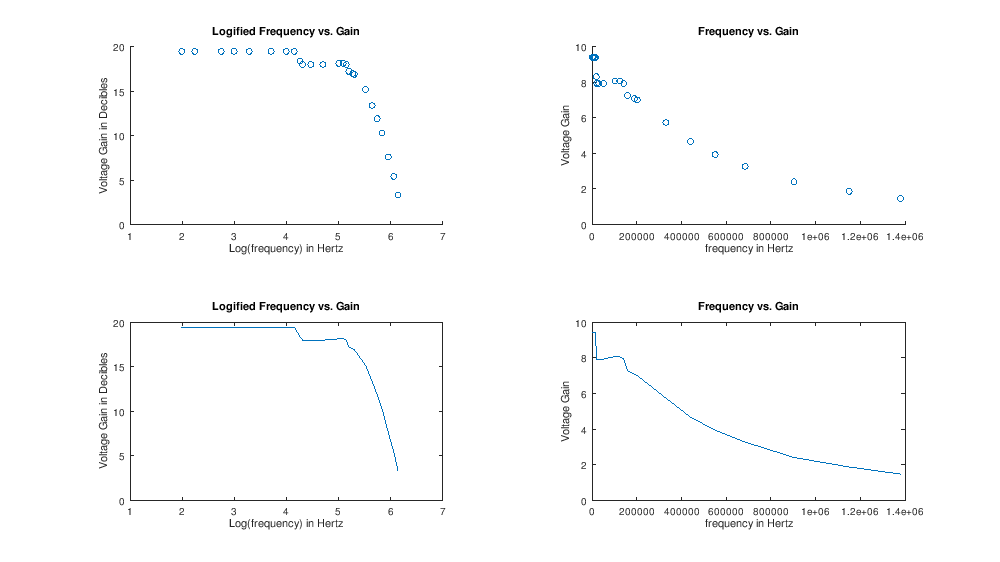
\includegraphics[width=7in]{bigGraph.png}
\caption{Frequency and Gain Voltages}
\label{fig1}
\end{figure}

The trend we are looking for in the Frequency vs. Gain is much easier to see when we logify both axes. If we also multiply the log of gain by 20 it conveniently becomes unit decibels. Above you can see the graphs both logified and pure. The left shows us the logified data that we expect to be similar to the Bode plot in the datasheet as seen below.

We do indeed see a similar curve but we ended up with two 'knees' in our data, instead of the one we expected. This could be due in part to a lack of data density around that location, but it seems that what data is there still shows the two bends. Perhaps this is a flaw within the op amp I used, a malfunction with my test equipment, or even human error in data recording.

One of the knees seems to fall around $log(f)=4.2$ and the other closer to $log(f)=5$. That puts these bends at roughly $f_{b1}=15850$, and $f_{b2}=100000$ respectively.

\begin{figure}[ht]
	\centering
	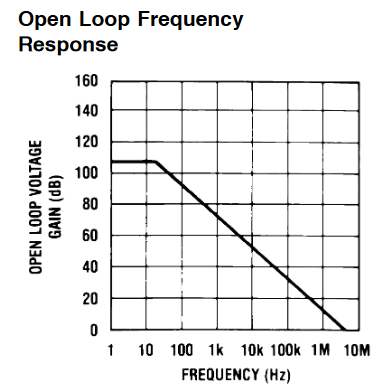
\includegraphics[width=3in]{datasheetBode.png}
	\caption{LF411 Open Loop Frequency Response Graph taken from LF411 Datasheet}
	\label{fig1}
\end{figure}

We can see in our logified graph that the second knee falls at around 17dB, which is 3db lower than our designed gain of 20dB. This much does match our expectations but I don't think it matches the Open Loop Frequency Response graph of the datasheet. If we follow our $f_{b1}$ and $f_{b2}$ up to find their respective $A_{OL}$ we find them to be roughly 30dB and 43dB. As stated earlier our design was meant to be a 20dB amplifier, so something isn't adding up here.

I'm not sure if I'm misunderstanding something, misinterpreting the graphs or data, created errors in either my math or data collection, didn't set up the amplifier correctly in the first place, or something entirely different, but I expected the bend to fall around 800kHz-1MHz, but I believe my data is showing it falling much sooner.

I did compare my data to others that also completed the experiment and while most only had one bend, the data mostly matched. This makes me think the experiment was likely not what went wrong.

\section{Analysis}
Not Requested

\begin{thebibliography}{99}
% The numeral (here 99) in curly braces is nominally the number of entries in
% the bibliography. It's supposed to affect the amount of space around the
% numerical labels, so only the number of digits should matter--and even that
% seems to make no discernible difference.
Not Requested
\end{thebibliography}

\end{document}
